\chapter{Estrategias de planificación de consultas}
\label{cap:planificacion}
Los motores de búsqueda verticales son diseñados con el propósito de lidiar con cargas de trabajos dinámicas. Un ejemplo de un motor de búsqueda vertical, es un motor de publicidad que ejecuta una consulta cada vez que un usuario abre un correo electrónico en por ejemplo, el servicio de \textit{Yahoo! mail}; de esta forma se muestra publicidad de acuerdo al contenido del correo electrónico. Eventualmente millones de usuarios concurrentes están conectados a sus correos electrónicos, por lo que la carga de trabajo esperada para el motor de búsqueda puede llegar a órdenes de las cien mil consultas por segundo \citep{Gil-Costa:2013}. Adicionalmente, el hecho que las actualizaciones en un motor de búsqueda vertical ocurran con mayor frecuencia que en uno de propósito general, hace que el diseño de los algoritmos para procesar las consultas sea diferente; también se debe permitir la actualización del índice invertido.

Por lo anteriormente mencionado, se hace imperioso tener un sistema diseñado que soporte altas cargas de trabajo, y las respuestas a consultas esten en una cota de tiempo aceptable para el usuario sin mermar la calidad de los resultados obtenidos. También es necesario que las estructuras de datos y algoritmos implementados soporten la concurrencia entre las transacciones de lecturas y escrituras; ya que eventualmente el motor de búsqueda tendrá que dejar de procesar consultas para poder servir las transacciones de escritura que actualizan el índice invertido.

A continuación se muestra las diferentes estrategias de planificación de transacciones de lectura abordadas en el presente trabajo utilizando diferentes enfoques; se presentan tres enfoques diferentes: El primero consiste en crear bloques de consultas en donde previamente a cada una de ellas se le asigna el número de hebras que utilizará en su resolución, luego el bloque es procesado en paralelo por los diferentes hilos de ejecución asignados; el segundo enfoque sirve de \textit{baseline}, cada hilo de ejecución se hace cargo de una consulta y lleva a cabo su procesamiento, en este enfoque la competencia entre los hilos de ejecución es por las consultas; El tercer y último enfoque corresponde a unidades de trabajos, en la que a cada transacción de lectura se le asigna un número determinado de unidades de procesamiento y los hilos de ejecución compiten por ellas obteniéndolas desde una cola.


\section{Estrategias por bloques}
\label{scheduling:bloques}
Un sistema de planificación de un motor de búsqueda trabaja en un contexto \textit{online}, esto significa que desconoce las transacciones que vendrán en el futuro y que cuando llega una nueva transacción de lectura, se debe tomar una decisión rápida acerca de qué hacer con ella. Adicionalmente, una transacción de lectura debe ser resuelta dentro de una cota superior de tiempo, al cual se llamará $t_{limite}$. En el contexto del presente trabajo, para que el planificador tome una decisión con respecto a una consulta, debe conocer de ella (1) su tiempo de ejecución y (2) el número de hebras con los que será resuelta. El tiempo de ejecución de cada consulta se obtiene utilizando los métodos de predicción de tiempos mostrados en el Capítulo \ref{cap:prediccion}; una vez que se predice el tiempo esperado $t_{esperado}$ de cada consulta para $1$,$2$,$4$,$8$ y $16$ hebras, se asigna el número de hilos de ejecución tal que se cumpla que $t_{esperado} < t_{limite}$, de esta forma se satisface la condición de que todas las consultas deben ser resueltas en una cota superior de tiempo previamente definida.

Bajo el contexto de un motor de búsqueda en el que se debe planificar transacciones de lecturas que eventualmente serán resueltas de forma paralela por diferentes hilos de ejecución, existe una estrategia teórica llamada FR que aborda este problema \citep{Ye:2007} y se adapta a este escenario de un motor de búsqueda vertical; esta estrategia del estado del arte da pie para que en el presente trabajo de tesis se proponga dos nuevas estrategias siguiendo el mismo enfoque de FR, pero estas enfocadas principalmente en mejorar la asignación de consultas a bloques, para así reducir el tiempo ocioso de las hebras. 

En la Figura \ref{fig:schedulerbloques} se muestra el proceso completo de este enfoque; las consultas que llegan al sistema las recibe el planificador (\textit{scheduler}) y las envía al estimador (\textit{estimator}), que calcula el número adecuado de hilos de ejecución para la consulta tal que ésta sea resuelta en un tiempo inferior al tiempo límite $t_{limite}$. Una vez que a la transacción de lectura se le predice el tiempo de ejecución y el número de hebras a utilizar, este planifica la consulta en algún bloque correspondiente depenediendo de la política que se este utilizando. A continuación se muestran las diferentes estrategias propuestas. 

\begin{figure}[!th]
\centering
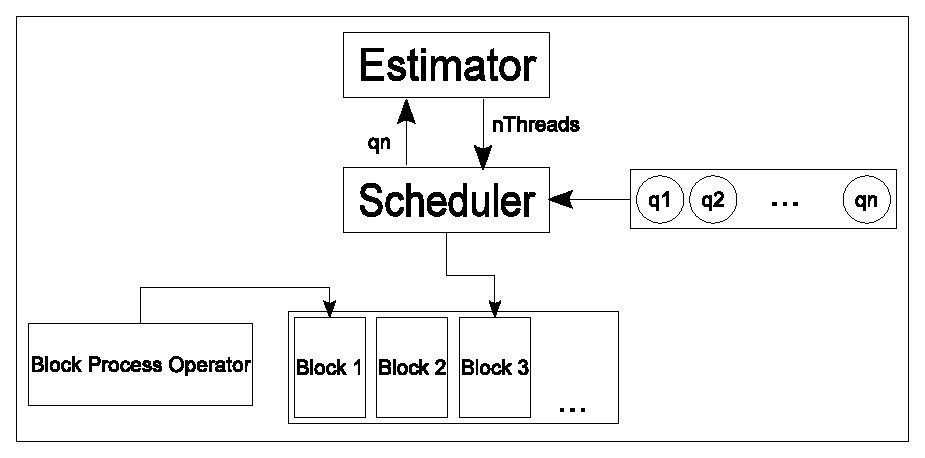
\includegraphics[scale=.75]{images/scheduler_bloques.eps}
\caption{Enfoque de planificación para estrategias por bloques.}
\label{fig:schedulerbloques}
\end{figure}  


\subsection{Estrategia FR}
\label{scheduling:fr}
La estrategia FR posee como requisito que cada una de las consultas a planificar se le haya asignado el número de hebras con las cuales se resolverá; esto se hará siguiendo el esquema \ref{fig:schedulerbloques}. Como se dijo anteriormente, a cada consulta se le asignará la cantidad mínima de hebras tal que el tiempo en resolver la consulta sea menor al tiempo límite $t_{limite}$.

Por lo explicado anteriormente, el algoritmo FR asume que cada consulta que llega al motor de búsqueda posee el número de hebras que debe utilizarse en su resolución. Utilizando esta información, la estrategia hace una clasificación de cada consulta entre \textit{Big} y \textit{Small}, con el objetivo de crear estructuras de datos denominadas \textit{Rooms} y {Walls}, en donde cada \textit{Wall} y cada {Room} estará formado solo por consultas de tipo \textit{Big} y \textit{Small} respectivamente. Ambas estructuras de datos tienen un número máximo de máquinas disponibles para procesar las transacciones de lectura. Una consulta es \textit{Big} si el número de máquinas requeridas para procesarla es $m$ (siendo \textit{m} el número de máquinas disponibles en el sistema), de lo contrario la consulta es \textit{Small}. La idea del algoritmo es crear bloques de consultas (\textit{Wall} y \textit{Room}), que serán procesadas en paralelo por el proceso que resuelve las consultas. 

Como se puede ver en el Algoritmo \ref{alg:fr}, cuando una nueva transacción de lectura llega al sistema, esta se analiza si es de tipo \textit{Big} o \textit{Small}; esto se hace en el método \textit{isBig()}, que retorna verdadero si es que el número de máquinas requeridas para procesar la consulta es igual al máximo de máquinas disponibles en el sistema, de lo contrario retorna falso y la transacción es clasificada como \textit{Small}. Si la consulta es \textit{Big}, entonces se crea una estructura de dato \textit{Wall}, se planifica la consulta en el bloque y esta se inserta en la lista de planificación \textit{SchedulingList} que contendrá todos los bloques con las consultas ya planificadas. Si se está en presencia de una transacción de lectura de tipo \textit{Small}, se busca algún bloque de tipo \textit{Room} para planificar esta consulta; para realizar lo anterior, el bloque debe satisfacer dos condiciones: (1) no debe estar completo, es decir, debe tener hebras disponibles, y (2) no debe haber sido procesado aún. Por último, si eventualmente no se encuentra algún bloque disponible para planificar la consulta, entonces se crea un nuevo bloque \textit{Room}, se planifica la consulta al bloque y este bloque es insertado en lista de \textit{scheduling}. Cabe destacar que se dice que un bloque está abierto (\textit{isOpen()}) cuando las consultas presentes en el bloque no han ocupado todos los hilos de ejecución disponibles o cuando el proceso de ejecución ya ha procesado el bloque. Es importante también notar que las estructuras de datos de tipo \textit{Wall} estarán formadas solo por una transacción de lectura de tamaño máximo.

\begin{algorithm}[!th]
\caption{\em $schedulerFR::assignQuery(L, Q)$: Planificación de consulta}
\label{alg:fr}
\begin{algorithmic}[1]
\REQUIRE Una SchedulingList $L$ en donde se hará la planificación, QueryObject $Q$ a planificar
\ENSURE SchedulingList $L$ con la nueva query planificada

\IF {$isBig(query)$}
	\STATE $block = new Wall();$
	\STATE $block \rightarrow addQuery(query);$
	\STATE $L \rightarrow addBlock(block);$
\ELSE
	\STATE $asignada = false;$
	\FOR {$ i = L \rightarrow firstOpenBlockLocked() ... L \rightarrow size()$}
		\STATE $room\_block = L \rightarrow getBlockLocked(i);$
		
		\IF {$(room\_block \rightarrow isOpen()) \& \& 
				(room\_block \rightarrow freeThreads() >= query \rightarrow getThreads())$
			}
			\STATE $room\_block \rightarrow addQuery(query)$
			\STATE $asignada = true$
			\STATE $break;$
		\ENDIF
	\ENDFOR
	
	\IF {$!(asignada)$}
		\STATE $block = new Room();$
		\STATE $block \rightarrow addQuery(query);$
		\STATE $L \rightarrow addBlockLocked(block);$		
	\ENDIF
\ENDIF

\end{algorithmic}
\end{algorithm}

En la Figura \ref{alg:fr} se presenta un ejemplo de ejecución la estrategia FR. Han llegado al sistema consultas: $q_{0}$ (2 hebras), $q_1$ (16 hebras), $q_2$ (4 hebras), $q_3$ (2 hebras), $q_4$ (2 hebras), $q_5$ (8 hebras) y $q_6$ (16 hebras). Se puede ver cómo se van formando las estructuras de datos llamadas \textit{Rooms} y \textit{Walls}. Suponer que eventualmente arriba al sistema una nueva consulta ($q_7$) que será resuelta con 8 hebras, entonces el algoritmo verifica en primera instancia la $Room_0$, sin embargo, en esta estructura no hay suficientes hilos de ejecución disponibles para procesar la consulta (posee solo 6 disponibles). Finalmente la planifica en la $Room_1$.

\begin{figure}[!th]
\centering
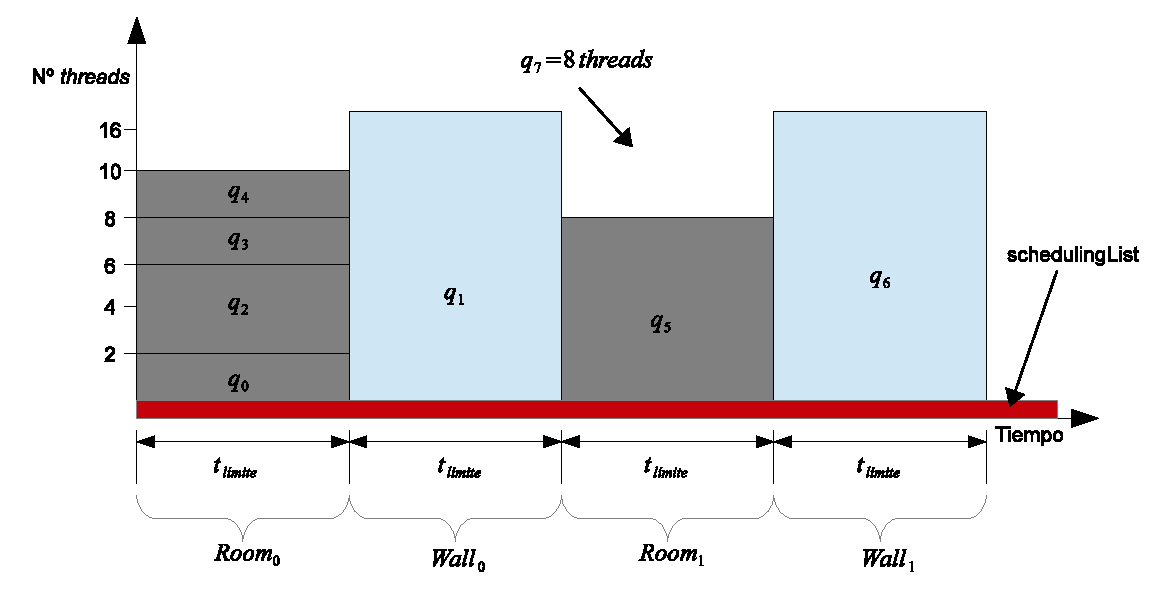
\includegraphics[scale=.75]{images/proceso_FR.eps}
\caption{Ejemplo de procesamiento de la estrategia FR.}
\label{fig:proceso_FR}
\end{figure} 

\subsection{Estrategia Times}
\label{scheduling:times}
Se intuye que una de las desventajas de la estrategia FR es que al planificar una consulta en algún bloque, solo verifica si es que este posee el número de hebras desocupados suficientes tal que sea mayor o igual al número de hilos requeridos por la consulta. Esto puede generar pérdida de eficiencia importante en los procesamientos de los bloques, puesto que algunas transacciones de lecturas pueden tomar mayor tiempo en ser procesadas y los hilos de ejecución que ya han terminado su trabajo estarán ociosos esperando por otros para continuar con el siguiente bloque. Para abordar esta posible pérdida de eficiencia, se diseña una política de planificación alternativa en donde además de tomar en cuenta el número de hebras disponible en cada bloque (como en la estrategia anterior), se toma en cuenta el tiempo esperado de la transacción de lectura.

Cada consulta $q$ tiene asociado un número de hilos de ejecución $NT_q$ y un tiempo $t_{predicho}$, que es el tiempo en que se espera que la consulta sea resuelta con $NT_q$ hilos de ejecución. La idea de esta estrategia es separar las transacciones de lectura que tengan tiempos de procesamiento muy diferentes en bloques distintos, es decir, se crearán bloques con consultas que tengan poca diferencia de tiempo unas de otra, de esta forma se quiere reducir el tiempo que se podría perder entre un bloque y otro por el desbalance de carga de los hilos. Cada bloque $B$ tendrá un tiempo $t_B$, que será el tiempo de la consulta con menor tiempo dentro del bloque. La métrica establecida para que una transacción de lectura que llega al sistema sea planificada en un bloque, es que el tiempo del bloque $t_B$ no sea el doble del tiempo de la consulta $t_q$ entrante, y viceversa. Si esta condición falla, entonces significa que la consulta $q$ que se está intentando planificar posee tiempos que se escapa a los rangos de tiempo del bloque $B$.

El Algoritmo \ref{alg:times} muestra el funcionamiento de la estrategia \textit{Times}, esta recibe como entrada la consulta a planificar y la lista de bloques (\textit{SchedulingList}). El algoritmo \textit{Times} trabaja de manera similar a la estrategia FR, la diferencia es que en esta estrategia una consulta puede ser planificada en un bloque siempre y cuando este tenga hebras disponibles suficientes para procesarla y que el tiempo de la consulta no doble al tiempo mínimo dentro del bloque perteneciente a alguna consulta ya planificada; si esta no puede ser planificada, entonces el bloque se desecha y se busca por otro bloque. Existirá un número limitado de bloques que se pueden desechar (\textit{$MAX\_BLOCKS\_CHECKED$}), si eventualmente se llega a este valor, se escoge aquel bloque con la mínima diferencia de tiempo con la consulta. En el peor de los casos, ningún bloque tendrá espacio suficiente para planificar la consulta y se deberá crear uno nuevo. Notar que en esta estrategia ya no se clasifican las consultas de acuerdo al número de hilos de ejecución que utilizan. 

\begin{algorithm}[!th]
\caption{\em $schedulerTimes::assignQuery(L, Q)$: Planificación de consulta}
\label{alg:times}
\begin{algorithmic}[1]
\REQUIRE Una SchedulingList $L$ en donde se hará la planificación, QueryObject $Q$ a planificar
\ENSURE SchedulingList $L$ con la nueva query planificada	
	\STATE $blocks\_viewed = 0$
	\STATE $blockValid = false;$	
	\STATE $best\_diff = INF;$	
	\FOR {$ i = L \rightarrow firstOpenBlockLocked() ... L \rightarrow size()$}
		\STATE $block = L \rightarrow getBlockLocked(i);$		
		\IF {$ block block \rightarrow freeThreads() \geq query \rightarrow getThreads() $}
			\STATE $tiempo\_min = block \rightarrow getMinimumTime()$			
			\IF {$ block \rightarrow isSchedulable(query) $}
				\STATE $L \rightarrow addQuery(query);$
				\STATE $assigned = true;$
				\STATE $break;$
			\ENDIF						
			\STATE $blocks\_viewed++;$			
			\IF {$blocks\_viewed \geq MAX\_BLOCKS\_CHECKED$}
				\STATE $break;$
			\ENDIF			
		\ENDIF		
	\ENDFOR	
	\IF {$ !(assigned)  \& \& (blocks\_viewed \geq MAX\_BLOCKS\_CHECKED) $}
		\STATE $block = new QueryBlock();$
		\STATE $block \rightarrow addQuery(query);$
		\STATE $L \rightarrow addBlockLocked(block);$		
	\ENDIF	
\end{algorithmic}
\end{algorithm}

En la Figura \ref{fig:proceso_Times} se muestra un ejemplo de la estrategia \textit{Times}, en el que una consulta llega al sistema y debe ser planificada. El estimador utilizado predijo que la transacción de lectura entrante se demorará 135 ms. con 8 hebras; en otras palabras, 8 hilos de ejecución es el número mínimo con el que se cumple que el tiempo de la consulta (135 ms.) es menor que la cota superior de tiempo (140 ms.). El algoritmo intenta planificar la consulta en primera instancia en el bloque $B_0$, sin embargo, el tiempo de la consulta (135 ms.) es el doble del mínimo tiempo en el bloque (55 ms.). Posteriormente, el bloque $B_1$ no posee hebras disponibles. Finalmente la transacción de lectura $q_7$ es planificada en el bloque $B_2$, ya que reúne todas las condiciones necesarias explicadas anteriormente en el algoritmo \ref{alg:times}. 

\begin{figure}[!th]
\centering
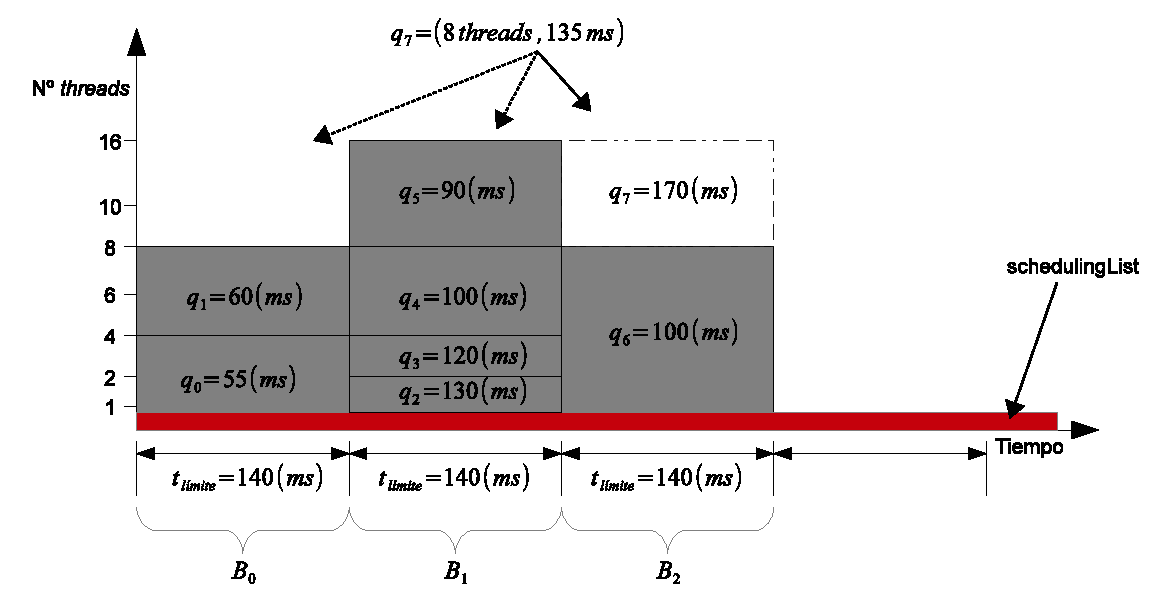
\includegraphics[scale=.75]{images/proceso_Times.eps}
\caption{Ejemplo de procesamiento de la estrategia Times.}
\label{fig:proceso_Times}
\end{figure} 

\subsection{Estrategia TimesRanges}
\label{scheduling:timesranges}
Esta estrategia también intenta disminuir la posible pérdida de eficiencia de la estrategia \textit{FR}. La idea de \textit{TimesRanges} es clasificar y agrupar las consultas de acuerdo a rangos de tiempos; para planificar una transacción de lectura que arriba al sistema, se debe encontrar un bloque que cumpla con: (1) número de hilos de ejecución libres suficientes, y (2) que el bloque sea del mismo rango de tiempo que la consulta. Inicialmente se define tres tipos de rangos: (1) aquellas que se demoren menos del 10\% del tiempo límite; (2) aquellas que se demoren más (o igual) del 10\% y menos del 25\% del tiempo límite; (3) aquellas que se demoren más (o igual) del 25\% y menos del 50\% del tiempo límite; y (4) aquellas que se demoren más (o igual) del 50\% del tiempo límite. De esta forma se reduce la diferencia de tiempos entre las consultas pertenecientes a un mismo bloque, lo que significa que consultas dentro de un mismo bloque deberían ser resueltas en tiempos muy parecidos. Recordar que el tiempo límite es la cota superior de tiempo en que una consulta debe ser resuelta.

El procedimiento de la estrategia \textit{TimesRanges} se puede ver en el algoritmo \ref{alg:timesranges}. Para que una transacción de lectura sea planificada bajo la presente estrategia, lo primero es obtener el rango de tiempo en que se encuentra la consulta entrante; posteriormente, se busca algún bloque que no haya sido procesado y que además posea un número de hebras disponibles suficiente para procesarla, y se planifica la consulta. Si no se encuentra un bloque que satisfaga las condiciones de la consulta entrante, entonces se crea uno nuevo para planificarla. 

\begin{algorithm}[!th]
\caption{\em $schedulerTimesRanges::assignQuery(L, Q)$: Planificación de consulta}
\label{alg:timesranges}
\begin{algorithmic}[1]
\REQUIRE Una SchedulingList $L$ en donde se hará la planificación, QueryObject $Q$ a planificar
\ENSURE SchedulingList $L$ con la nueva query planificada	
	\STATE $range = getQueryRange(query);;$		
	\FOR {$ i = L \rightarrow firstOpenBlockLocked() ... L \rightarrow size()$}
		\STATE $block = L \rightarrow getBlockLocked(i);$	
		\IF {$ block block \rightarrow freeThreads() \geq query \rightarrow getThreads() \& \&  block_ranges[i] == range$}
			\STATE $block = L \rightarrow addQuery(query);$
			\STATE $asignada = true;$
			\STATE $break;$	
		\ENDIF
	\ENDFOR
	\IF {$ !(asignada) $}
		\STATE $block = new QueryBlock();$	
		\STATE $block->addQuery(query);$	
		\STATE $L \rightarrow addBlockLocked(block);$
		\STATE $block_ranges[L \rightarrow size - 1] = range;$	
	\ENDIF
\end{algorithmic}
\end{algorithm}


\section{Estrategia \textit{1TQ}}
\label{scheduling:baseline}
Un simple camino para construir un sistema que responda a múltiples consultas simultáneamente usando múltiples hilos de ejecución, es usando estos hilos de manera independiente. Para hacer esto se debe mantener un conjunto de hilos de ejecución consumidores que trabajarán en paralelo y se encargarán de resolver las transacciones de lectura secuencialmente (una a una) desde una misma cola, esto es lo que en este trabajo se denomina estrategia de Un Thread Por Query (1TQ). En la Figura \ref{fig:1TQ} se puede apreciar el esquema de ejecución en donde cada uno de los procesos genera una petición de alguna consulta en la cola, si quedan consultas por procesar entonces se le asigna al proceso una consulta que tendrá que resolver de manera secuencial. Se debe tener en cuenta que cada vez que un proceso genera una solicitud de consulta, se bloquea la estructura de datos que contiene las consultas a procesar y luego se procesa la solicitud, de esta forma se asegura un acceso seguro por parte de los distintos hilos de ejecución. 

\begin{figure}[H]
\centering
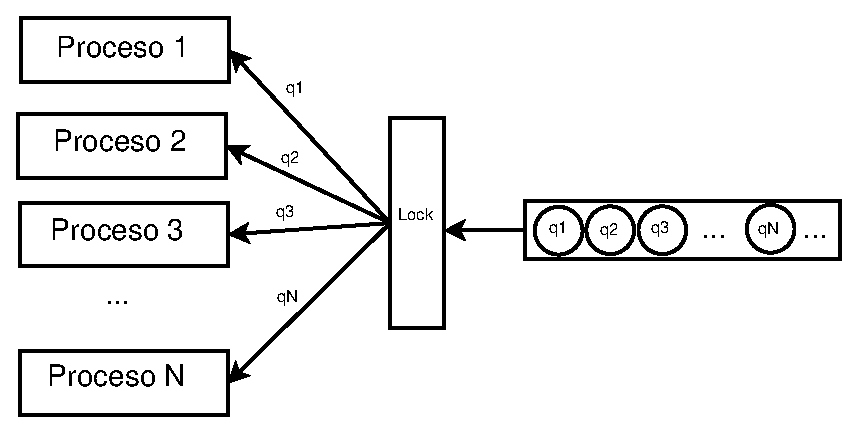
\includegraphics[scale=.75]{images/1TQ.eps}
\caption{Ejemplo de procesamiento estrategia 1TQ.}
\label{fig:1TQ}
\end{figure}

Este esquema tiene la ventaja que es simple y fácil de implementar y controlar. Sin embargo, existen sistemas de recuperación de información como los motores de búsqueda verticales que cuando están ejecutando \textit{batches} de consultas deben parar su ejecución porque transacciones de escritura han llegado al sistema, y estos deben actualizar la información del índice invertido. Solo después de la fase de actualización el sistema es capaz de ejecutar el siguiente \textit{batch} de transacciones de lectura. Al final de cada conjunto de consultas, es posible que algunos hilos de ejecución del sistema finalicen su trabajo y que no tengan más consultas para procesar, por lo que ellos tienen que esperar que los hilos restantes finalicen su trabajo antes que el sistema entre en la fase de actualización de su índice invertido o bien, se pase a la ejecución del siguiente \textit{batch} de consultas.
Sin embargo, aunque cada hilo de ejecución está secuencialmente ejecutando una transacción de lectura diferente, algunas de estas operaciones puede tomar un tiempo cosiderable, de esta forma se produce una importante pérdida de eficiencia, aunque la intuición nos dice que esto se puede mitigar con transacciones de lectura que requieran poca cantidad de tiempo para ser procesadas (trabajos pequeños o \textit{small jobs}). 
En la Figura \ref{fig:small_jobs} queda reflejado lo dicho en el párrafo anterior. Si los trabajos que cada \textit{thread} está ejecutando son pequeños, entonces probablemente la pérdida de trabajo al final de cada \textit{batch} de consultas será menor al trabajo que se pierde cuando los trabajos son grandes (ver Figura \ref{fig:large_jobs}).  

\begin{figure}[H]
\centering
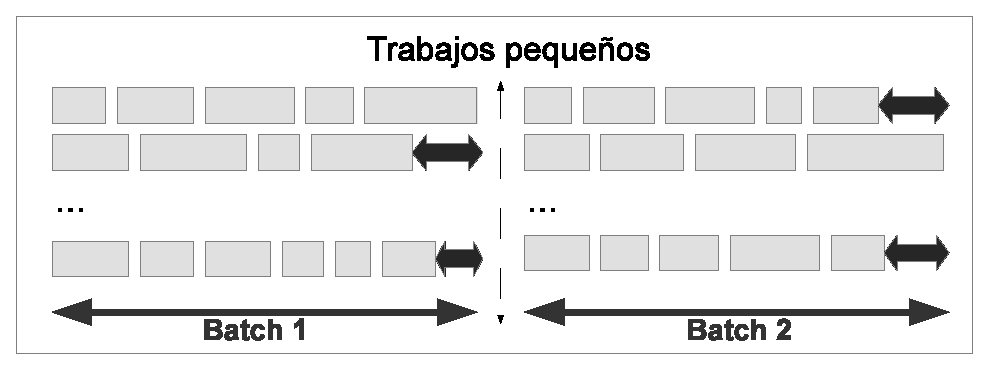
\includegraphics[scale=.75]{images/small_jobs.eps}
\caption{Ejecución en paralelo de \textit{small jobs}.}
\label{fig:small_jobs}
\end{figure}

\begin{figure}[H]
\centering
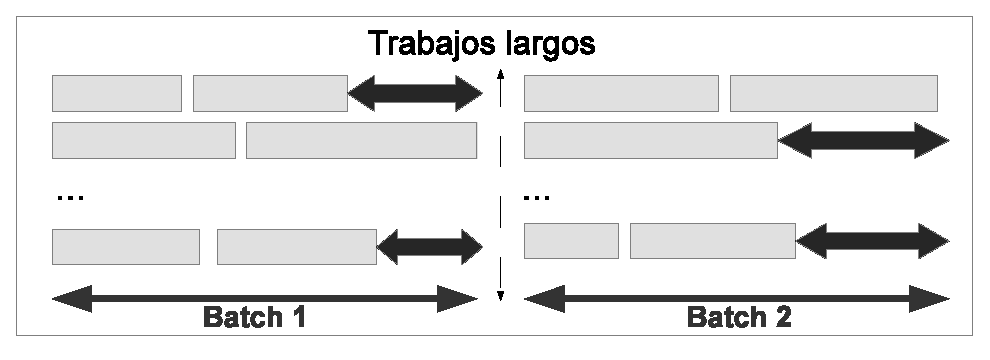
\includegraphics[scale=.75]{images/large_jobs.eps}
\caption{Ejecución en paralelo de \textit{large jobs}.}
\label{fig:large_jobs}
\end{figure}


\section{Estrategia unidades de trabajo}
\label{scheduling:unidadestrabajo}
Con respecto a los esquemas explicados hasta ahora, el esquema 1TQ tiene la ventaja que no solo requiere menos control, sino que también permite a los hilos de ejecución trabajar sin pausa mientras se resuelven transacciones de lectura por lotes; sin embargo, no se garantiza una cota superior de tiempo para cada consulta. En esta sección se propone un esquema en donde la consulta es dividida en unidades de procesamiento o de trabajo, en el que a cada unidad se le asigna la parte del índice invertido con el cual se debe trabajar. Además existe un nivel de datos compartido entre las unidades de procesamiento, como por ejemplo, el \textit{heap} en donde se guardará el conjunto \textit{top-K}.

En este nuevo esquema de planificación, las consultas pasan a través de una fase en la cual se predice sus tiempos de ejecución y se le asigna el mínimo número de hebras tal que se cumpla con la cota superior de tiempo establecida. Posteriormente se estima para cada consulta el número de unidades de procesamiento que se utilizará en su resolución, este número será igual al número de hilos de ejecución estimado (Ver Figura \ref{fig:unit_process}). Un conjunto de hilos consumidores extraen las unidades desde la cola y las procesan de forma independiente. Cuando una hebra finalice el procesamiento de la unidad de trabajo actual, automáticamente extraerá la siguiente unidad de trabajo desde la cola. De esta forma se forma una competencia entre los hilos de ejecución por las unidades de trabajo de la cola, por lo que se debe controlar el acceso concurrente de los hilos al nivel compartido de datos entre las unidades de procesamiento, de tal manera que solo una hebra tenga acceso exclusivo a este objeto para poder actualizar los datos a medida que cada una de las unidades de la transacción de lectura es resuelta.


\begin{figure}[!th]
\centering
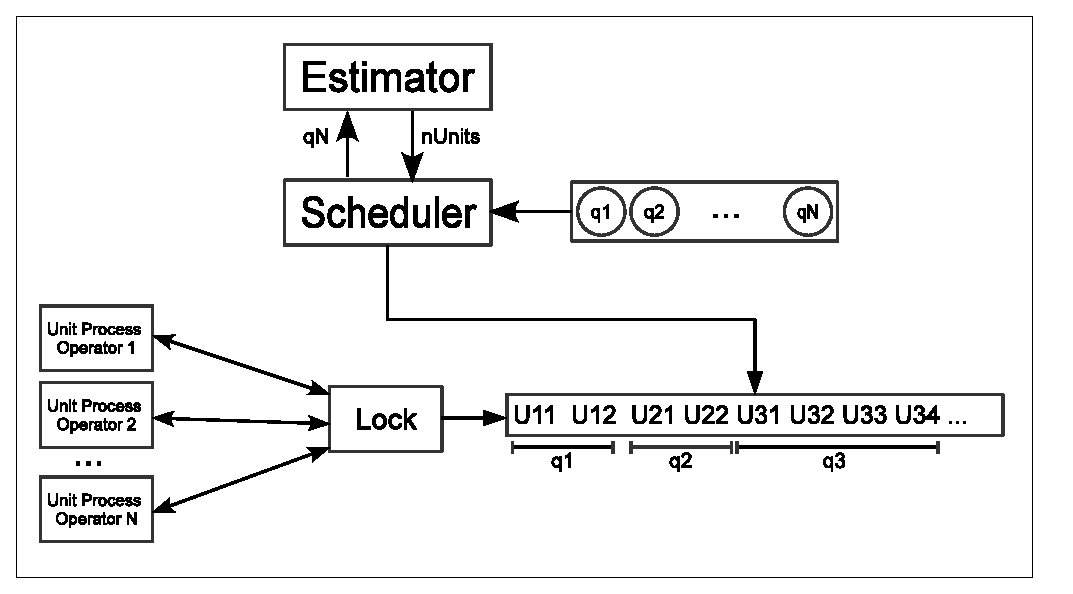
\includegraphics[scale=.75]{images/unit_process.eps}
\caption{Procesamiento de consultas utilizando unidades de trabajo.}
\label{fig:unit_process}
\end{figure}

Se muestra un ejemplo en la Figura \ref{fig:queryunit_execution} en el que se resuelven cuatro consultas. La consulta 0 fue dividida en cuatro unidades de trabajo; la consulta 1 y 2 en dos unidades de trabajo; y finalmente la consulta 3, en ocho unidades de trabajo. Los hilos de ejecución competirán por la extracción de unidades de trabajo desde la lista.

\begin{figure}[!th]
\centering
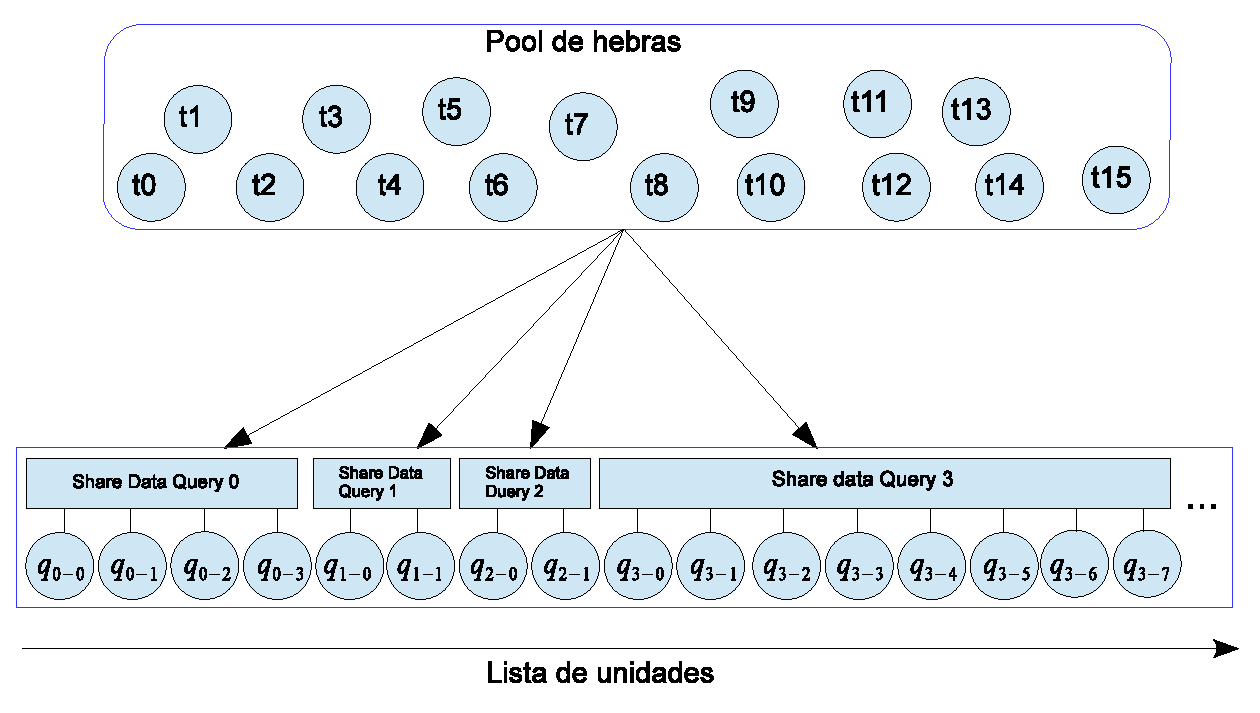
\includegraphics[scale=.75]{images/QueryUnitExecution.eps}
\caption{Esquema de ejecución estrategia unidades de procesamiento.}
\label{fig:queryunit_execution}
\end{figure}

El procesamiento de cada hilo de ejecución es una versión de Wand con \textit{heap} compartido (SH), adaptado de manera tal que cada unidad de trabajo es resuelta independientemente de si existen otras unidades siendo procesadas al mismo tiempo. La única excepción es que la unidad de procesamiento que inicializa la consulta es siempre ejecutada antes del resto de las otras unidades de la misma consulta, y también la entrega de resultados se hace una vez que todas las unidades de procesamiento de la consulta han finalizado. Este enfoque híbrido permite reducir el tiempo perdido al final de cada \textit{batch} de consultas sin generar una importante pérdida de trabajo mientras las consultas del \textit{batch} están siendo procesadas.

En la Figura \ref{fig:queryunit_scheduler} se presenta el diagrama de clases del planificador de unidades de procesamiento:

\begin{list}{}{}
	\item \textbf{TopKMultiThreadWandOperatorLocal}. Clase encargada de devolver los mejores $K$ documentos para una transacción de lectura dada. Si es que la consulta debe ser resuelta en forma paralela, esta clase además debe controlar el paralelismo que se produce en la resolución de ésta, inicializando las variables correspondientes para lanzar los hilos de ejecución y luego escogiendo los mejores documentos desde todos los heaps creados por los diferentes hilos (proceso de \textit{merge}). En esta clase se define un mapa que asocia cada término del índice invertido con el puntaje del mejor documento en esa lista invertida (\textit{upper bound} de la lista invertida) y además se define cuántos documentos se van a retornar al final del proceso (atributo $K$). El método \textit{execute} inicializa las variables locales para las diferentes hebras, posteriormente hace el llamado al método \emph{thread-execute} (en el cual se llevará a cabo la resolución de la transacción de lectura en forma paralela), finalmente se toman los resultados parciales de cada uno de los hilos de ejecución y se ejecuta el proceso que mezcla los resultados, retornando solo los mejores $K$ documentos. 
	
	\item \textbf{QueryObject}. Clase que representa las transacciones de lectura a las que se le asignará unidades de procesamiento.
	
	\item \textbf{QueryUnit}. Clase que representa las unidades de procesamiento de transacciones de lectura. Cada uno de estos objetos tiene asociado un nivel de datos compartido (QueryUnitShareData) con otras unidades de procesamiento que resolverán la misma consulta.
			
	\item \textbf{QueryUnitShareData}. Clase que permite la creación de datos compartidos entre las unidades de procesamiento. Todas las variables compartidas por las unidades de trabajo estarán albergadas en este objeto. 
	
	\item \textbf{QueryEstimator}. Clase que se encarga de estimar el número de unidades de procesamientos requeridas para una cierta consulta.
	 
	\item \textbf{QueryUnitScheduler}. Clase principal del planificador, esta se encarga de tomar las transacciones de lectura y asignarle a cada una de ellas el número de unidades de procesamiento adecuado. Finalmente, las unidades de trabajo de planifican en una lista.
\end{list}

\begin{figure}[!th]
\centering
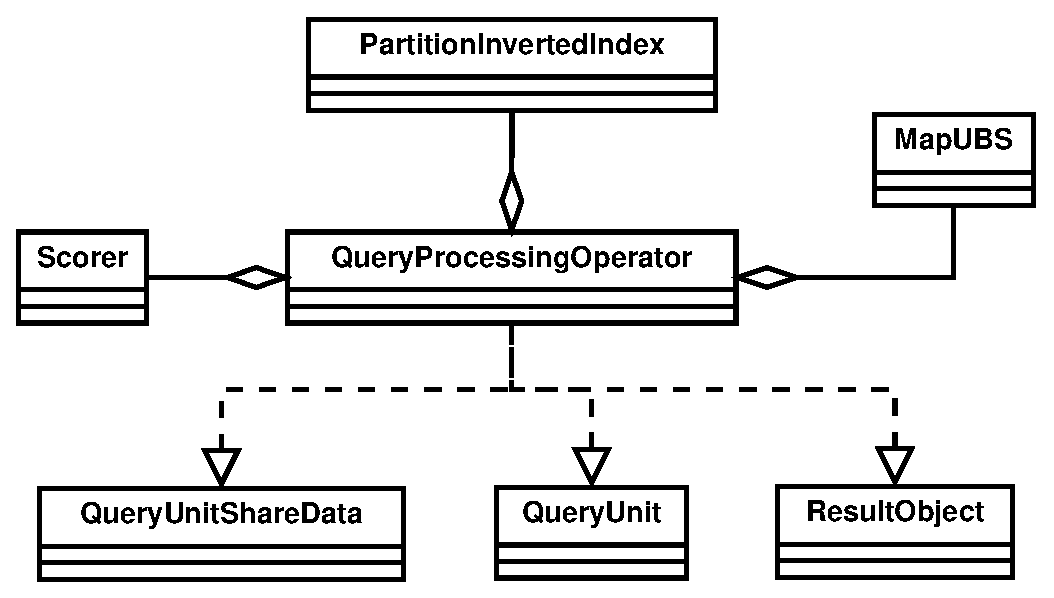
\includegraphics[scale=.75]{images/QueryUnitExecuter.eps}
\caption{Diagrama de clases del ejecutador de unidades de procesamiento.}
\label{fig:queryunit_scheduler}
\end{figure}

Finalmente se diseña un diagrama de clases para el ejecutador de unidades de procesamiento (Ver Figura \ref{fig:queryunit_scheduler}). Aquí se puede observar los objetos involucrados en la resolución de cada consulta; cada objeto QueryProcessingOperator es el encargado de procesar una unidad, y habrán tantos objetos de este tipo como hilos de ejecución disponibles en el sistema. Cada vez que una unidad es procesada, si es que restan unidades por resolver, el hilo de ejecución toma inmediatamente la siguiente unidad de trabajo, de lo contrario debe retornar el conjunto final de documentos que se encuentra en el \textit{heap} compartido. 

\begin{figure}[!th]
\centering
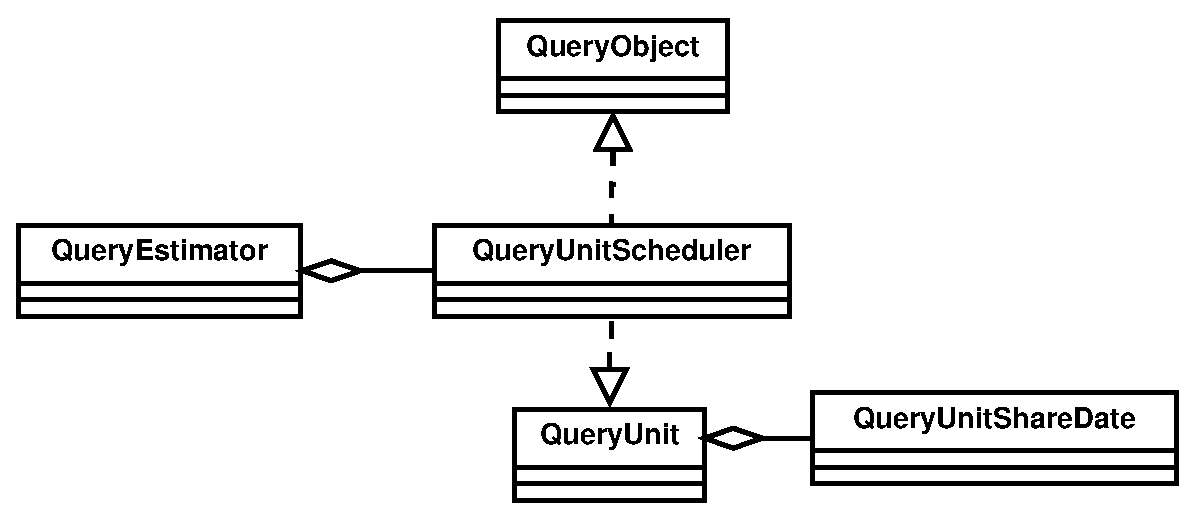
\includegraphics[scale=.75]{images/QueryUnitScheduler.eps}
\caption{Diagrama de clases del planificador de unidades de procesamiento.}
\label{fig:queryunit_scheduler}
\end{figure}